\documentclass{beamer}
\usetheme{default}
\usepackage{multicol}
\usepackage{amsmath,amssymb,amsthm}
\usepackage{diffcoeff}
\usepackage{bm}
\usepackage[most]{tcolorbox}
\usepackage{subcaption}
\usepackage[backend=bibtex, style=authoryear, doi=false,isbn=false,url=false]{biblatex}
\usepackage{color}
\definecolor{theme}{RGB}{0,73,114}

\newcommand{\inpr}[3][]{\ensuremath{\langle #2, \, #3 \rangle_{#1}}}
\newcommand{\dualpr}[3][]{\ensuremath{\langle #2 \, \vert #3 \rangle_{#1}}}


\graphicspath{{./images/}}
\bibliography{biblio_pres}

\setbeamertemplate{blocks}[rounded][shadow]

\setbeamercolor{block body alerted}{bg=alerted text.fg!10}
\setbeamercolor{block title alerted}{bg=alerted text.fg!20}
\setbeamercolor{block body}{bg=structure!10}
\setbeamercolor{block title}{bg=structure!20}
\setbeamercolor{block body example}{bg=green!10}
\setbeamercolor{block title example}{bg=green!20}


% Remove navigation bar
\setbeamertemplate{navigation symbols}{}
%\addtobeamertemplate{navigation symbols}{}{%
%	\usebeamerfont{footline}%
%	\usebeamercolor[fg]{footline}%
%	\hspace{1em}%
%	\insertframenumber/\inserttotalframenumber
%}

\newif\iftocsub
\tocsubtrue
\AtBeginSection[] {
	\begin{frame}[noframenumbering]{Outline}
		\tableofcontents[sectionstyle=show/shaded, subsectionstyle=show/show/hide]
	\end{frame}
	\tocsubfalse
}
\AtBeginSubsection[] {
	\iftocsub
	\begin{frame}[noframenumbering]{Outline}
		\tableofcontents[currentsubsection, sectionstyle=show/shaded, subsectionstyle=show/shaded/hide]
	\end{frame}
	\fi
	\tocsubtrue
}

\newcommand{\beginbackup}{
	\newcounter{framenumbervorappendix}
	\setcounter{framenumbervorappendix}{\value{framenumber}}
}
\newcommand{\backupend}{
	\addtocounter{framenumbervorappendix}{-\value{framenumber}}
	\addtocounter{framenumber}{\value{framenumbervorappendix}} 
}


\title{Projet MORPHEUS}
\author{Andrea Brugnoli}
\begin{document}
\begin{frame}[plain]
    \maketitle
\end{frame}

\begin{frame}{Overview}
	\tableofcontents
\end{frame}

\section{Modelling multiphysical systems with Hamiltonian dynamics}

\begin{frame}{Modelling framework for the MORPHEUS project}
	
	\begin{block}{Main objective}
		Use a unified port-Hamiltonian (pH) framework to model fluid-structure interactions.
	\end{block}
	
	If successful, the approach will: 
	\begin{itemize}
		\item be competitive w.r.t. state of the art methods;
		\item pave the way to other multiphysical problems;
		\item serve for model reduction and control of complex systems.
	\end{itemize}
	
	\begin{figure}[t]
		\begin{subfigure}[t]{0.3\textwidth}
			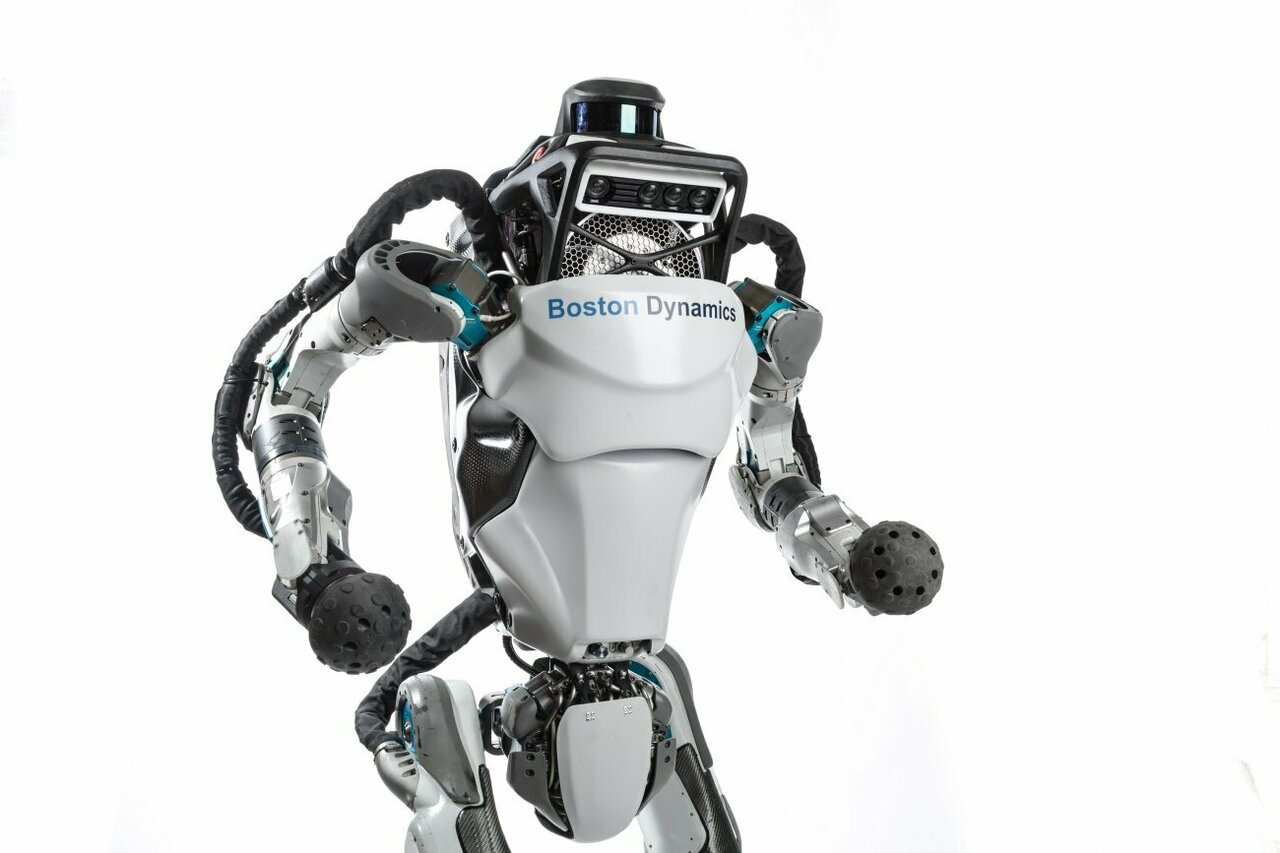
\includegraphics[width=\columnwidth]{robotics.jpg}\\
			\centering{Robotics}%
		\end{subfigure}\hfill
		\begin{subfigure}[t]{0.3\textwidth}
			
\includegraphics[width=\columnwidth]{aerospace.jpg}\\
			\centering{Aerospace} 
		\end{subfigure}\hfill
		\begin{subfigure}[t]{0.3\textwidth}
			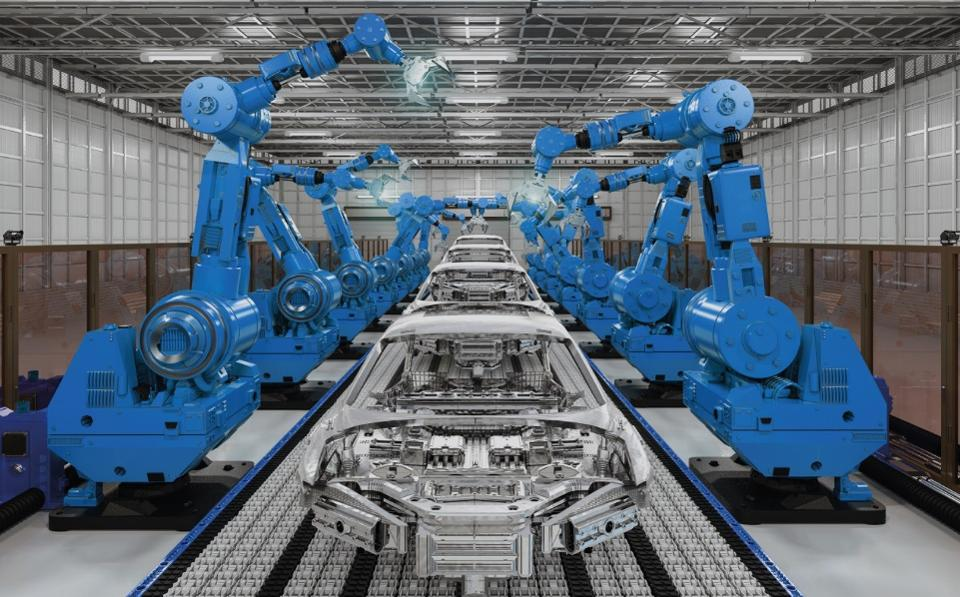
\includegraphics[width=\columnwidth]{manufacturing.jpg}\\
			\centering{Manufacturing}
		\end{subfigure}
	\end{figure}

\end{frame}



\begin{frame}{Why port-Hamiltonian systems?}
		\begin{columns}
			\begin{column}{.45\textwidth}
				\begin{figure}
					\centering
					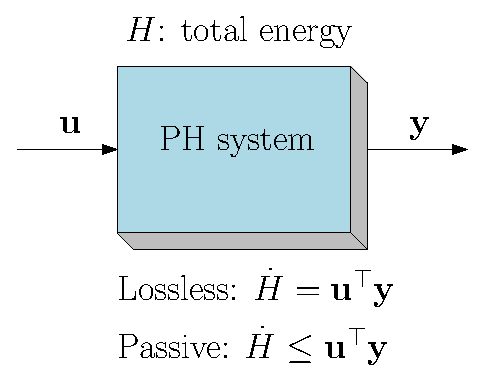
\includegraphics[width=.95\textwidth]{sketch_PH.eps}
				\end{figure}
			\end{column}
			\hspace{1cm}
			\begin{column}{.5\textwidth}
				PH systems are:
				\begin{itemize}
					\item Physically motivated;
					\item Lumped (ODEs) or distributed (PDEs);
					\item Passivity based control;
					\item \textcolor{theme}{Closed under interconnection (modular multiphysics modelling)};
				\end{itemize}
			\end{column}
		\end{columns}	
	
\end{frame}

\begin{frame}{Energy preserving interconnection of pHs}
	\only<1>{
		\begin{figure}
			\centering
			\includegraphics[width=.95\textwidth]{sketch_PH_gyrator.eps}
		\end{figure}
	}
	\only<2>{
		\begin{figure}
			\centering
			\includegraphics[width=.95\textwidth]{sketch_PH_transformer.eps}
		\end{figure}
	}
	
\end{frame}


\begin{frame}{Distributed port-Hamiltonian systems}
	
	\begin{block}{General structure}
		
		$H(\bm{\alpha})$ is the Hamiltonian functional:
		\begin{equation*}
			\begin{aligned}
				\partial_t {\bm{\alpha}} &= (\mathcal{J} - \mathcal{R}) \, \bm{e}, \\
				\bm{e} &:= \only<1>{\delta_{\bm{\alpha}}{H}}, \\
				\bm{u}_\partial &= \mathcal{B}_\partial  \, \bm{e}, \\
				\bm{y}_\partial &= \mathcal{C}_\partial \, \bm{e}, 
			\end{aligned} \qquad
			\begin{aligned}
				\bm{\alpha} &\quad\text{State variables},\\
				\bm{e} &\quad\text{Effort variables},\\
				\bm{u}_\partial &\quad\text{Boundary control input}, \\
				\bm{y}_\partial &\quad\text{Collocated output}. 
			\end{aligned}
		\end{equation*}
	Operators:
	\begin{itemize}
		\item $\mathcal{J}$ Interconnection operator (skew-symmetric);
		\item $\mathcal{R}$ Dissipation operator (semi-positive definite);
		\item $\mathcal{B}_\partial$ Boundary input operator; 
		\item $\mathcal{C}_\partial$ Boundary output operator. 
	\end{itemize}
	Energy balance:
	\begin{equation*}
	 \dot{H} = \dualpr{\bm{u}_\partial}{\bm{y}_\partial} - \inpr{\bm{e}}{\mathcal{R}\bm{e}} \le \dualpr{\bm{u}_\partial}{\bm{y}_\partial}
	\end{equation*}
	\end{block}
	
	
\end{frame}



\section{A unified discretization framework for port-Hamiltonian systems}


\begin{frame}{The MORPHEUS project and its numerical challenges}
	Numerical methods for multiphysical systems should:
	\begin{itemize}
		\item reproduce the physical properties of the problem (conservation laws, symmetries);
		\item work in any spatial dimension and coordinate frame;
		\item distinguish between the dynamics and the constitutive equations;
		\item adaptable to many physical problems (fluid and solid mechanics, electromagnetism, etc.);
		\item preserve the exchanges of energy flow for different physical domain;
	\end{itemize}
\end{frame}

\begin{frame}{Methods for computational simulation}
	\begin{itemize}
		\item Finite differences (Taylor expansion of derivatives);
		\item Finite volumes (Integral form of the equations);
		\item Finite elements (Variational formulation of the PDE);
	\end{itemize}
\vspace{1cm}
If the constructions stem from the same ideas, these schemes may be completely equivalent:\\
\fullcite{adler2021}

\end{frame}

\begin{frame}{What to choose for port-Hamiltonian systems?}
	Two important questions:
		\begin{itemize}
			\item Can we rely on established theoretical results to have a clear guideline and unified analysis of different methods?
			\item Can we rely on existing and robust software packages? 
	\end{itemize}
	
\end{frame}


\begin{frame}{Exterior calculus and discretization of PDEs}
	
	\begin{block}{A unified discretization framework}
		\fullcite{arnold2006acta}
	\end{block}
	
	This framework comes with a periodic table of finite elements for unified analysis\footnote{\url{https://sinews.siam.org/Details-Page/periodic-table-of-the-finite-elements}}.
	
	\begin{figure}[t]
		\begin{subfigure}[t]{0.23\textwidth}
			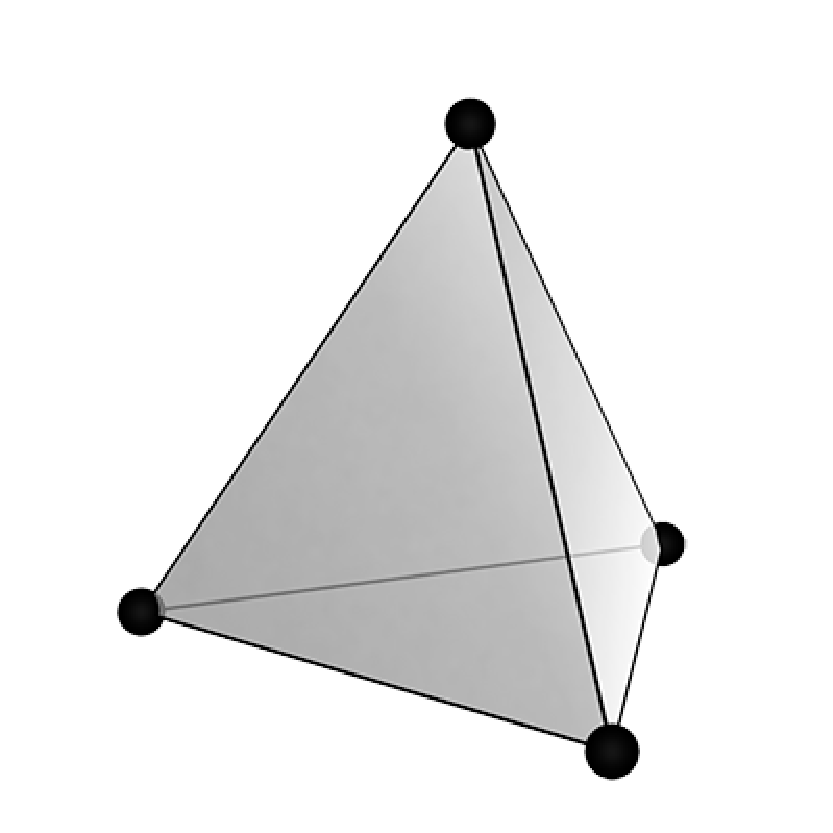
\includegraphics[width=\columnwidth]{P1_tetrahedron.pdf}%
		\end{subfigure}
		\begin{subfigure}[t]{0.23\textwidth}
			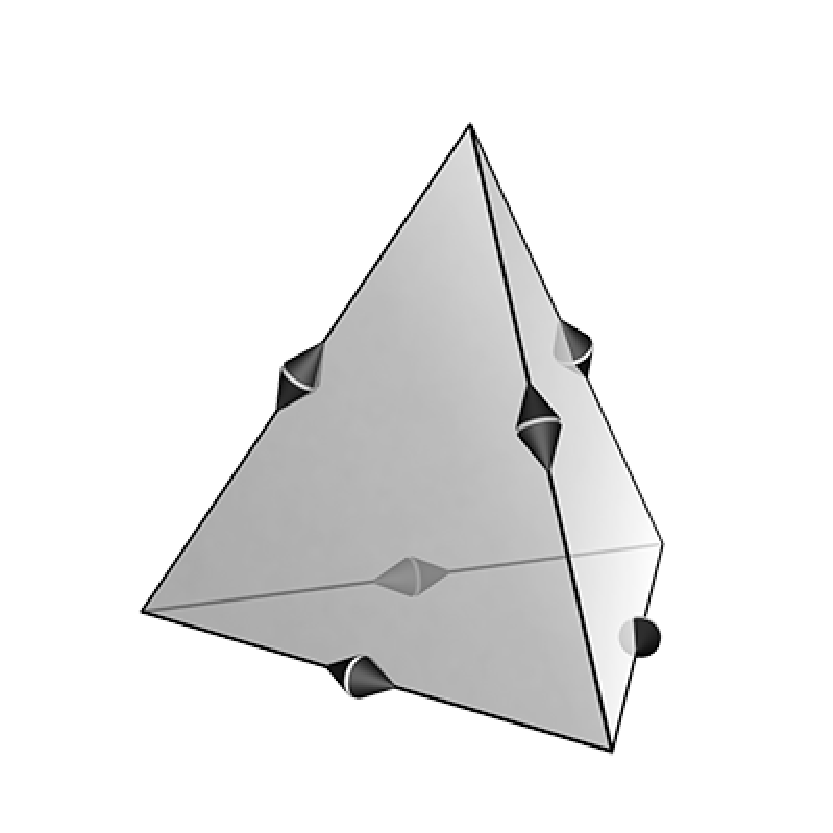
\includegraphics[width=\columnwidth]{N1e1_tetrahedron.pdf}%
		\end{subfigure}\hfill
		\begin{subfigure}[t]{0.23\textwidth}
			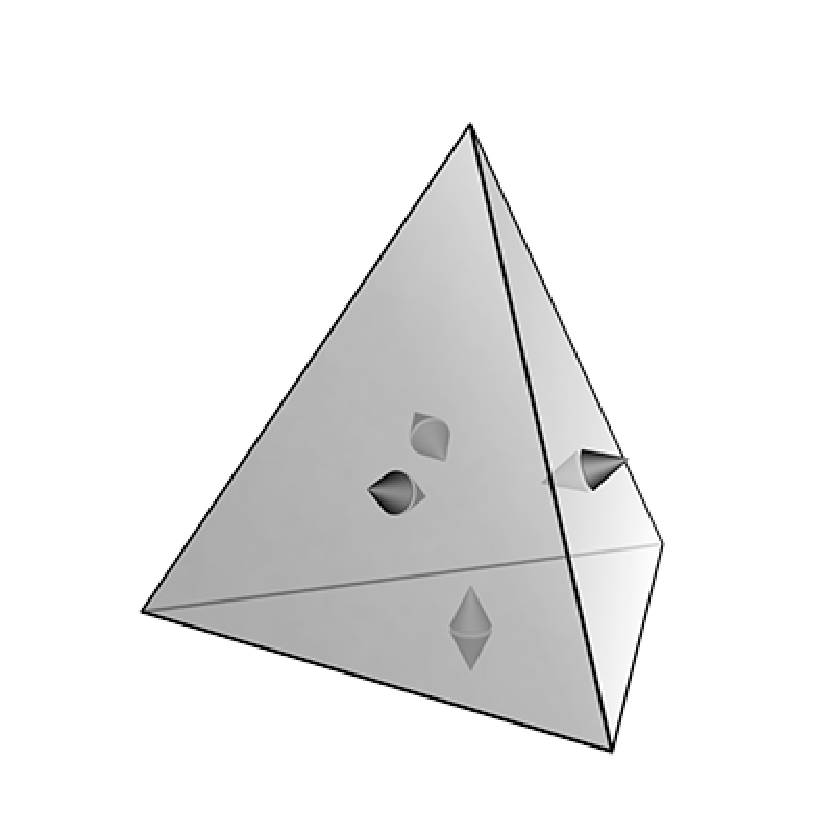
\includegraphics[width=\columnwidth]{N1f1_tetrahedron.pdf}%
		\end{subfigure}\hfill
		\begin{subfigure}[t]{0.23\textwidth}
			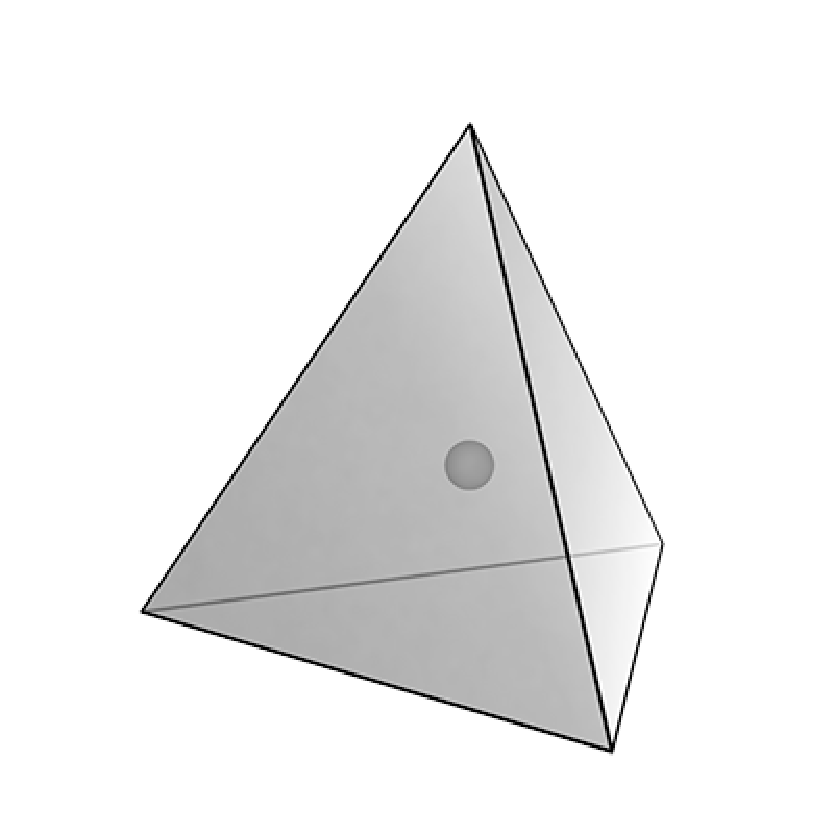
\includegraphics[width=\columnwidth]{dP0_tetrahedron.pdf}%
		\end{subfigure}\hfill
	\caption{The $\mathcal{P}^-_1\Lambda^k$ family (Whitney forms 1957)}
	\end{figure}
\end{frame}

\begin{frame}{The impact of FEEC}
	\begin{block}{On the importance of FEEC}
		\textit{"Just as the arrangement of the chemical elements in a periodic table led to the discovery of new elements, the periodic table of finite elements has not only clarified existing elements but also highlighted holes in our knowledge and led to new families of finite elements suited for certain purposes."}
	\end{block}
 This theory was employed successfully for:
	\begin{itemize}
	\item Electromagnetism;
	\item Fluid-Mechanics;
	\item Solid Mechanics.
	\end{itemize}
	Two open source libraries were built to implement the FEEC periodic table\footcite{logg2012,rathgeber2017firedrake}.
\end{frame}


\section{Artificial Intelligence for Model Order Reduction}

\begin{frame}{Artificial intelligence for Model Order Reduction (MOR)}


High dimensional full order system
\begin{equation*}
	\dot{\mathbf{x}} = \mathbf{f}(\mathbf{x}, \mathbf{p}), \qquad \mathbf{x} \in \mathbb{R}^n, \; n \gg 1
\end{equation*}
\begin{itemize}
	\item $\mathbf{x}$ State vector;
	\item $\mathbf{p}$ Parameters vector (boundary conditions, materials etc.).
\end{itemize}
How to obtain a reduced order model
\begin{equation*}
	\dot{\mathbf{x}}_r = \mathbf{f}_r(\mathbf{x}_r, \mathbf{p}), \qquad \mathbf{x}_r \in \mathbb{R}^r, \; r \ll n
\end{equation*}
valid for the whole parameter space $\mathbf{p}$ using IA and NN?

\end{frame}

\begin{frame}{An IA architecture for Galerkin and Petrov-Galerkin MOR}
	\fullcite{lee2020}
	\begin{figure}[t]
		\begin{subfigure}[t]{0.465\textwidth}
			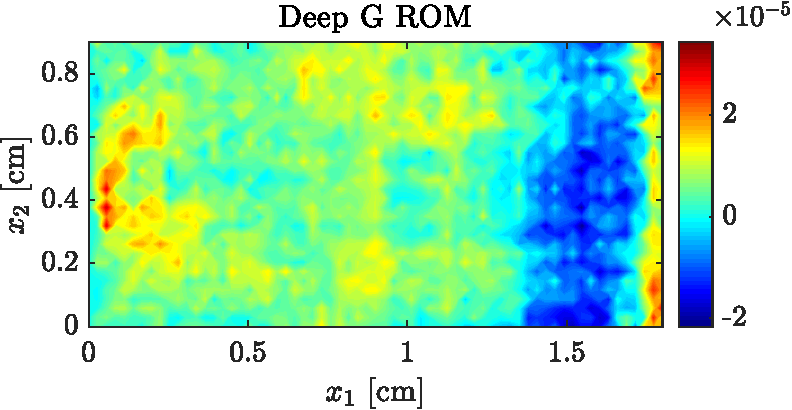
\includegraphics[width=\columnwidth]{DGROM_T_param1.pdf} 
			\caption{Reduced model with IA.}
		\end{subfigure}\hfill
		\begin{subfigure}[t]{0.48\textwidth}
			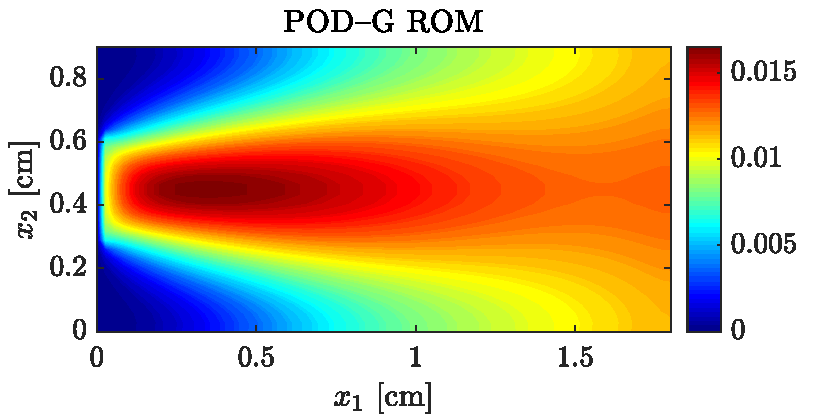
\includegraphics[width=\columnwidth]{GROM_T_param1.pdf}%
			\caption{Reduced model with POD.}
		\end{subfigure}
		\caption[]{Error of reduced models on the temperature field for a problem of convection-diffusion-reaction. By using a convolutional neural network to generate a nonlinear manifold (left) the error associated with the reduction is drastically reduced, from $10^{-2}$ to $10^{-5}$, compared to the POD method (right).}%
	\end{figure}
\end{frame}

\begin{frame}{Extension to port-Hamiltonian systems}
	\begin{itemize}
		\item How to incorporate physical structure in the Neural Network architecture?
		\item What if the system is interconnected to other components or actively controlled?
	\end{itemize}
\end{frame}




\end{document}
